\documentclass[a4paper]{article}

%% Language and font encodings
\usepackage[english]{babel}
\usepackage[utf8x]{inputenc}
\usepackage[T1]{fontenc}

%% Sets page size and margins
\usepackage[a4paper,top=3cm,bottom=2cm,left=3cm,right=3cm,marginparwidth=1.75cm]{geometry}

%% Useful packages
\usepackage{amsmath}
\usepackage{graphicx}
\usepackage[colorinlistoftodos]{todonotes}
\usepackage[colorlinks=true, allcolors=blue]{hyperref}

\title{Reporte de Actividad 5: Preparando datos con ayuda de Emacs}
\author{Jesús Antonio González Espinosa \\ \\ Física Computacional 1}
\date{Martes, 6 de Marzo del 2018}

\begin{document}
\maketitle

\section{Introducción}
En este reporte se presentan el proceso y los resultados de la actividad 5, donde trabajamos con herramientas ya estudiadas en actividades previas, así como nuevas. El trabajo de esta semana consistió en reutilizar los datos de la activida 4; los cuales limpiamos y filtramos mediante otros scripts y con el uso de el editor Emacs. Finalmente, con ayuda de Python, se presentará un análisis de los resultados obtenidos de los datos CAPE y PW de el Observatorio de Valentia.

Anterior  esto, explicaremos los conceptos de CAPE y PW, para poder entender qué son los datos con los que se trabajan; así como un desarrollo de como se hizo la actividad. Sin más preámbulos, iniciemos explicando los conceptos.


\section{Conceptos Físicos}
Ahora se dará una descripción de los conceptos CAPE y PW.

\subsection{CAPE}
Convective Available Potential Energy o CAPE es una herramienta muy útil para determinar el potencial de climas severos en cualquier lugar, en cualquier momento. Es un indicador de inestabilidad atmosférica. 
CAPE es la cantidad de energía boyante disponible para acelerar un parcel verticalmente, o la cantidad de trabajo que hace un parcel en el ambiente. Entre más alto sea el valor del CAPE, más energía habrá para que crezca una tormenta. En el momento en que la masa de aire se vuelve inestable, esta se desplaza hacia arriba de forma acelerada, causado por la diferencia de presión del aire desplazado y el aire ambiente en la altitud a donde se movió. Esto causa que se formen nubes por convección, que eventualmente crean tormentas. 
La unidades de medida es de $J/Kg$. Y en la siguiente tabla mostramos los valores que puede adquirir y su clasificación en estabilidad.
\begin{center}
 \begin{tabular}{||c | c||} 
 \hline
 CAPE & Potencial  \\ [0.5ex] 
 \hline\hline
 0 & Estable \\ 
 \hline
 0 - 1000 & Marginalmente Inestable \\
 \hline
 1000 - 2500 & Moderablemente Inestable \\
 \hline
 2500 - 3500 & Muy Inestable \\
 \hline
 3500 +  & Extremadamente Inestable \\ [1ex] 
 \hline
\end{tabular}
\end{center}

\subsection{PW}
Precipitable Water (PW) o agua precipitable, es el indicador de humedad que hay a partir de un punto fijo. Esto ayuda a dar una idea de la humedad en el aire; por lo que un valor elevado, indica mayor posibilidad de lluvia. El agua precipitable se mide en milímetros o pulgadas. A continuación, una tabla para haceros una idea de la cantidad de humedad según su medición, en pulgadas. 
\begin{center}
 \begin{tabular}{||c | c||} 
 \hline
 Cantidad & Humedad  \\ [0.5ex] 
 \hline\hline
 0.5 - & Muy baja humedad \\ 
 \hline
 0.5 - 1.25 & Baja humedad \\
 \hline
 1.25 - 1.75 & Humedad Moderada \\
 \hline
 1.75 - 2 & Alta humedad \\
 \hline
 2 +  & Muy alta humedad \\ [1ex] 
 \hline
\end{tabular}
\end{center}

Por otra parte, el agua precipitable total (TPW) es la cantidad de agua que se puede obtener, en un una columna de sección transversal de unidad que va desde la tierra hasta los límites de la atmósfera, si todo el vapor y el agua que contiene se condensara a forma liquida. 

\section{Proceso de Limpieza}
Para el proceso de limpieza, primero tomamos el archivo de la actividad pasada, df2017.cs, que contiene todos los datos del Observatorio de Valentia del año 2017. Ahora, en un script damos instrucción de filtrar todas las líneas que contengan las palabras clave "03953", "CAPE" y "PRECIP"  con un comando \textit{grep} y lo mandaremos a un archivo nuevo llamado df2017CAPE\_PW.csv. 

\begin{figure}[h!]
 \centering
  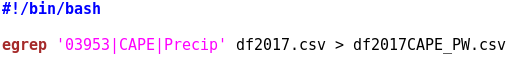
\includegraphics[width=0.4\textwidth]{script1.png}
\end{figure}

Estas palabras clave nos va a guardar, entre vario texto innecesario, los datos de las fechas, CAPE y PW respectivamente, que es con lo que se quiere trabajar. 
 \smallskip
Ahora, para limpiar esa basura que hay entre los datos, podemos usar Emacs, ya que esa basura está de forma repetitiva a través de todo el archivo. Entonces, lo abrimos con Emacs e iniciamos la limpieza, para esto, es un proceso muy simple: 
 \begin{enumerate}
 \item con ctrl + espacio, nos permite seleccionar, por lo que seleccionamos lo que deseamos borrar.
  \item con ctrl + w borramos lo seleccionado y queda guardado en junk.
   \item con ctrl + y pegamos lo que haya en junk, devolviendo el texto borrado en el paso anterior.
    \item volvemos al inicio del texto con ctrl + <, y abrimos el query replace con esc +  \%. El query replace es el que nos va a permitir remplazar texto dentro del archivo.
     \item ahora, pegamos ahí lo que tenemos con ctrl + y, y remplazamos eso en todo el archivo con nada (lo dejamos en blanco).
      \item finalmente usamos !, lo que va a hacer que se haga esta sustitución en todo el texto, borrando lo que insertado a remplazar. 
 \end{enumerate}
Repetimos estos pasos hasta dejar solo la fecha y los datos de CAPE y PW. En algunas repeticiones hubo que sustituir el texto por una coma, en vez de nada, para poder separar los datos y sean legibles por Pandas. Con esto, resulta un archivo que contiene dos datos por día de cada mes, uno de 00Z y otro de 12Z. Lo que hacemos con esto es hacer un script nuevo que filtre todo lo que tenga 00Z en un archivo y lo que tenga 12Z en otro. 

\begin{figure}[h!]
 \centering
  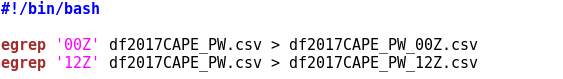
\includegraphics[width=0.4\textwidth]{script2.png}
\end{figure}

Ahora, esto nos da como resultados dos archivos: df2017CAPE\_PW\_00.csv y df2017CAPE\_PW\_12.csv. Abrimos cada uno con emacs y repetimos el proceso enumerado arriba para borrar el texto "00Z" y "12Z" de sus respectivos archivos. Con esto, obtenemos los datos separados, ordenados y listos para ser utilizados en Pandas. 

\section{Análisis de Datos}

Abrimos Jupyter Notebook, y como ya lo hemos hecho antes, preparamos las librerías necesarias. Usamos las bibliotecas de Pandas, Numpy y una nueva llamada datetime. Éste último sirve para cambiar el formato de la fecha. Ahora leemos los archivos de datos y convertimos la columna que contiene los datos de CAPE de objeto a número. También le damos encabezado a cada columna y con el comando df.head() lo imprimimos en pantalla. Repetimos este proceso para ambos archivos, con los datos de 00Z y 12Z:

\begin{figure}[ht!]
 \centering
  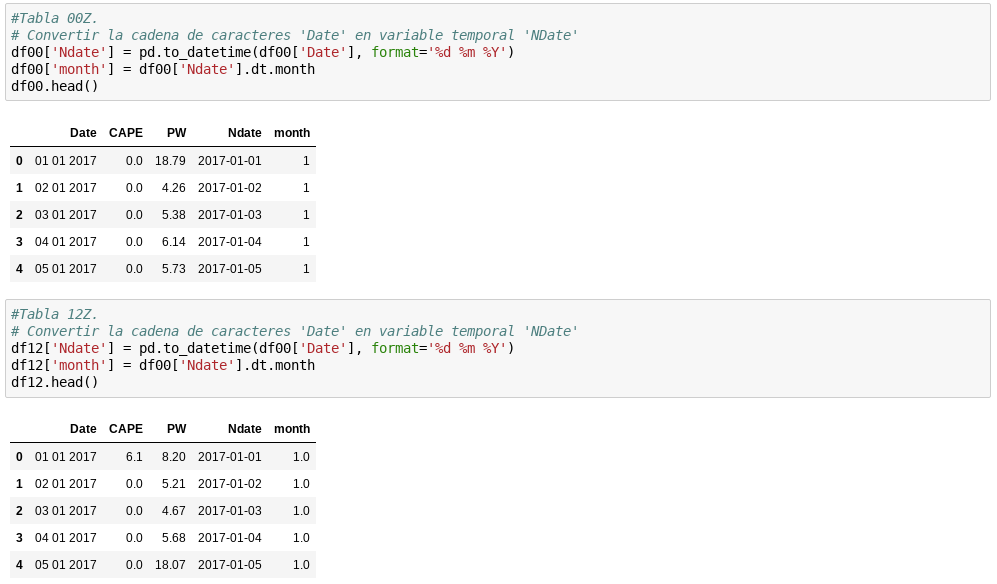
\includegraphics[width=0.6\textwidth]{DF1.png}
\end{figure}

Ahora, arreglamos los datos de la columa de las fechas, ya que ésta está siendo considerada como una cadena de caracteres, haciendo que no lo trabaje como otro dato. Haciendo uso de la nueva bibloteca, datetime, podemos convertirlo en lo que es, un dato de tipo fecha. De nuevo, repetimos este proceso para los dos archivos:

\begin{figure}[ht!]
 \centering
  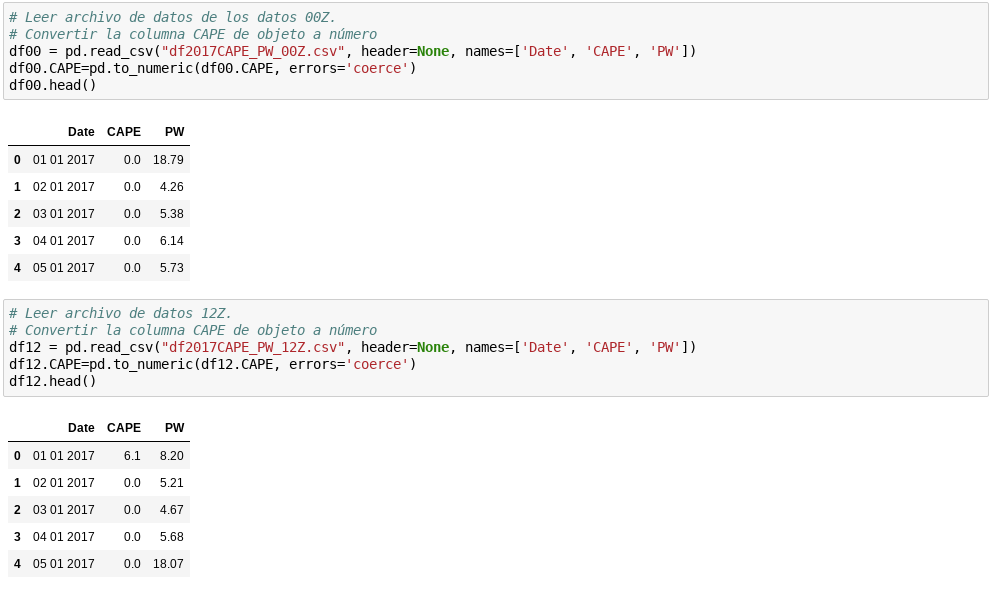
\includegraphics[width=0.6\textwidth]{DF2.png}
\end{figure}

Con esto, los datos están listos para ser graficados para poder observarlos y analizarlos. En la siguiente sección, vamos a ver nuevos tipos de gráficas para poder dar una descripción de la información que aportan.  

\pagebreak
\section{Resultados}

Primero, vamos a presentar gráficas de tipo Boxplot, donde se presentan 4 gráficas: las primeras dos siendo de los datos CAPE contra los 12 meses del año, una siendo de la hora 00Z y de 12Z respectivamente; y las siguientes dos siendo de los datos PW contra los 12 meses del año, de igual forma, uno siendo de la hora 00Z y de 12Z respectivamente.

\begin{figure}[ht!]
 \centering
  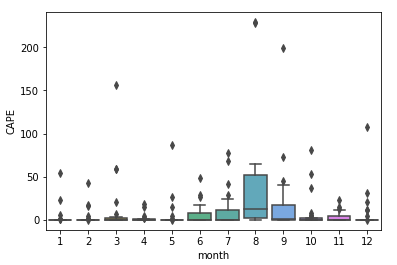
\includegraphics[width=0.6\textwidth]{00Z_Boxplot_CAPE.png}
  \caption{CAPE - Meses en 00Z}
\end{figure}
\begin{figure}[ht!]
 \centering
  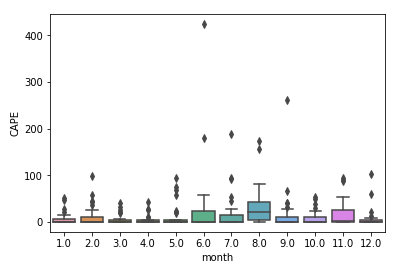
\includegraphics[width=0.6\textwidth]{12Z_Boxplot_CAPE.png}
  \caption{CAPE - Meses en 12Z}
\end{figure}

Con las gráficas de tipo Boxplot podemos observar varios datos importantes; en este caso del CAPE, podemos ver que en todos los meses, casi todos los valores están en 0, haciendo que la caja resulte muy pequeña y la media esté sesgada de forma muy drástica. También podemos ver un caso especifico, en el mes 8 (Agosto), donde en 00Z los datos aún siguen sesgados pero hacía abajo dentro de la caja; y en 12Z parecen estar más centrado en el rango intercuantílico, pero siendo una caja más pequeña.

\pagebreak
\begin{figure}[ht!]
 \centering
  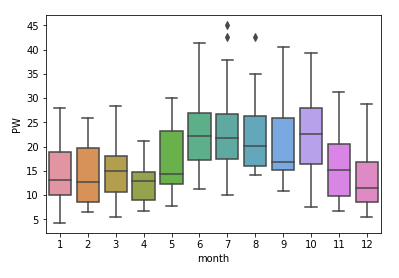
\includegraphics[width=0.6\textwidth]{00Z_Boxplot_PW.png}
  \caption{PW - Meses en 00Z}
\end{figure}
\begin{figure}[ht!]
 \centering
  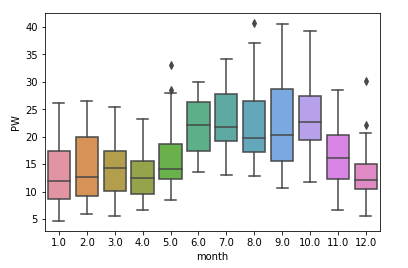
\includegraphics[width=0.6\textwidth]{12Z_Boxplot_PW.png}
  \caption{PW - Meses en 12Z}
\end{figure}

En el caso de los Boxplots de los datos PW en los 12 meses del año, vemos cajas más grandes y medias más centralizadas a excepción de unos meses como el, 4 (Abril), 5 (Mayo) y 9 (Septiembre) en los datos del 00Z; y los meses 1 (Enero), 2 (Febrero), 5 (Mayo), 7 (Julio) y 8 (Septiembre)  en el caso de los datos del 12Z. También podemos observar como entre los meses de 6 al 10, las cajas suelen estar más arriba. 

\pagebreak
Ahora se muestran las gráficas de los datos PW contra CAPE, para ver la relación que hay entre ellas.

\begin{figure}[ht!]
 \centering
  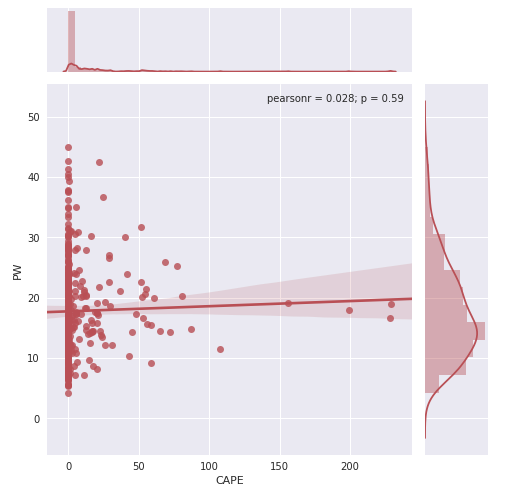
\includegraphics[width=0.6\textwidth]{00Z_Joinplot.png}
  \caption{PW - CAPE en 00Z}
\end{figure}
\begin{figure}[ht!]
 \centering
  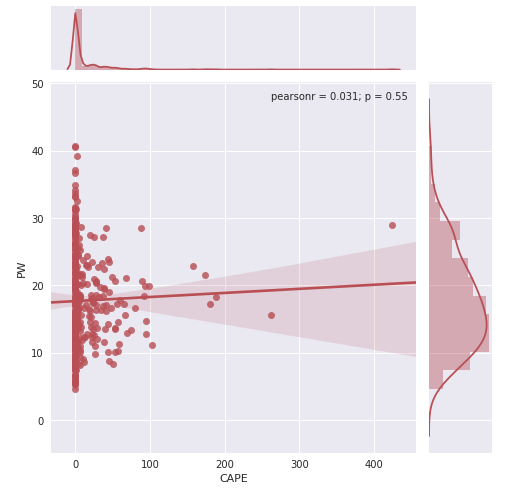
\includegraphics[width=0.6\textwidth]{12Z_Joinplot.png}
  \caption{PW - CAPE en 12Z}
\end{figure}

En este caso, en la parte superior podemos observar la distribución de los datos de CAPE y a la derecha la distribución de PW, mientras que la gráfica principal, que muestra CAPE en función de PW. muestra la recta que se ajuste mejor a los datos. Podemos observar que en ambas gráficas, 00Z y 12Z, las distribuciones son muy parecidas, y el ajuste muestra no haber ninguna relación entre los datos, ya que estos están muy dispersos y concentrados a la izquierda. 

\pagebreak
Finalmente, tenemos dos gráfica, una de los datos 00Z y otra de 12Z, con 12 rectas cada una, representando cada mes. 
\begin{figure}[ht!]
 \centering
  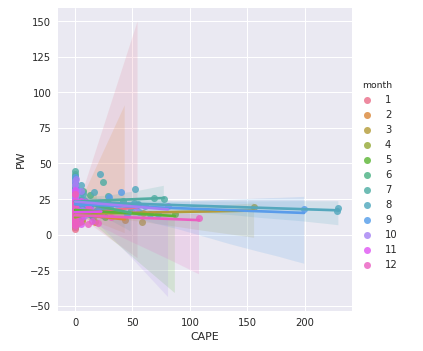
\includegraphics[width=0.6\textwidth]{00Z_Lmplot.png}
  \caption{PW - CAPE en 00Z}
\end{figure}
\begin{figure}[ht!]
 \centering
  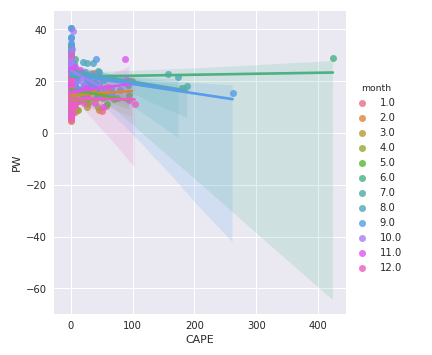
\includegraphics[width=0.6\textwidth]{12Z_Lmplot.png}
  \caption{PW - CAPE en 12Z}
\end{figure}

Como ya se acaba de mencionar, podemos de ver que cada recta pertenece a cada mes, mostrando la información relacionado los datos CAPE con PW. También podemos ver que en cada una de esas rectas se forman triángulos, los cuales representan la distribución de los datos de cada mes. Podemos observar que en ambos, todos los triángulos apuntan hacía abajo; con la excepción de dos de los primeros meses de 00Z. 


\pagebreak
\section{Conclusiones}

La actividad ha sido interesante, ya que hemos juntado un poco de lo que se ha visto en las cuatro actividades previas: desde Pandas con las librerías  y unas nuevas, hasta scripts para organizar los datos, además de otras herramientas vistas  anteriormente. También, como siempre, aprendimos sobre nuevos conceptos físicos, en este caso, sobre el CAPE y el PW.

Con este trabajo se pudo reafirmar lo concluido de una actividad anterior donde se dijo que lo más complicado de interpretar los datos era la parte de la limpieza; aunque en esta actividad todo fue muy rápido, pero en comparación, eso llegó a ser lo más tardado. Finalmente, podemos concluir en que los resultados fueron satisfactorios de acorde a la actividad, y eso se puede ver reflejado en este reporte.

\section{Bibliografía}
\begin{enumerate}
\item American Meteorological Society (2015) \textit{Precipitable Water}. Recuperado el 4 de Marzo del 2018 desde http://glossary.ametsoc.org/wiki/Precipitable\_water

\item Haby, J. (s.f.) \textit{What is Precipitable Water?} Recuperado el 4 de Marzo del 2018 desde http://www.theweatherprediction.com/habyhints3/899/

\item American Meteorological Society (2017) \textit{Conective Available Potential Energy}. Recuperado el 4 de Marzo del 2018 desde http://glossary.ametsoc.org/wiki/Convective\_available\_potential\_energy

\item WeatherOnline (s.f.) \textit{CAPE - Convective Available Potential Energy}. Recuperado el 4 de Marzo del 2018 desde https://www.weatheronline.co.uk/reports/wxfacts/CAPE---Convective-Available-Potential-Energy.htm
\end{enumerate}

\section{Apéndice}
\begin{enumerate}
\item \textbf{¿Cómo se te hizo esta actividad? ¿Compleja, Difícil, Sencilla?}

Al principio pareció que iba a ser una actividad muy difícil y compleja, pero resultó ser sencilla ya que entendías los conceptos con los que se había que trabajar.

\item \textbf{¿Qué te llamó más la atención?}

Me llamó la atención la facilidad que trajo Emacs al limpiar datos. A comparación de la actividad 3, donde usamos Pandas, en Emacs el proceso fue mucho más fácil.

\item \textbf{¿Qué parte fue la que menos te interesó hacer?}

Los scripts, ya que por alguna razón, me tomó tiempo poder hacerlos que corrieran correctamente. Además de que hay algunos conceptos que no tengo muy claros en como funcionan o como usarlos; pero son dudas menores.

\item \textbf{¿Cómo mejorarías esta actividad? ¿Qué le faltó? ¿Qué sobró?}

La actividad no le faltó nada, en realidad fue muy divertida y rápida una vez que se entendieron los conceptos y el proceso de limpieza en Emacs. El tiempo fue suficiente y las instrucciones fueron muy claras.


\item \textbf{¿Hasta este punto, que te parece el uso de Jupyter para programar en Python?}

Me ha gustado mucho, porque siento mucha comodidad en su entorno, es muy estético y simple, a comparación de Fortran, que es el lenguaje que más "domino" en la programación.

\end{enumerate}
\end{document}